% !TeX root = ../BA_main_englisch.tex
% !TeX spellcheck = en_GB
In this section we examine the higher-dimensional case of $N=5$.
As the data set with $\rho_0 = \ket{+} \bra{+}$, the eigenstate of the drive Hamiltonian $H_{(D)S}$, performed best in the previous section, we focus our attention on this case.
We compare the efficiency of a fully-connected ANN (FCANN) to a unidirectional and bidirectional LSTM to analyse the effect of different architectures on the predictive power in our setting.
Both LSTM networks have the same architecture, bar the bi-directionality (see Figure \ref{lstm_network}).
This hyperparameter distinguishes the two cases of whether or not the complete drive sequence is known in advance.

Before entering the LSTM cell, each embedded $\ket{\psi_D^n}$ passes through two fully-connected layers to increase the input dimensionality and add non-linearities to the input.
After passing the LSTM a single fully-connected layer is applied to the output to produce the embedding size (Eq. (\ref{embedding})) to recover $\ket{\psi_T^n}$.

\begin{figure}[h]
	\centering
	\includegraphics[width=0.75\textwidth]{img/lstm_network}
	\caption{Architecture of the LSTM networks. The green blocks represent the unidirectional case. For the bidirectional case, a second LSTM block (orange) is included with separate trainable parameters. Each LSTM block includes multiple layers of LSTM cells. The blocks labelled `FC' represent fully-connected layers.}
	\label{lstm_network}
\end{figure}

The FCANN is made up of three fully-connected hidden layers, the size of which are selected to approximately match the amount of trainable parameters of the bidirectional LSTM.

The test data efficiency as well as the amount of trainable parameters are presented in Table \ref{n5efftable}.

\begin{table}[h]
	\centering
	\begin{tabular}{ c | c | c | c | c}
		Network Architecture & $\eta_{test} \ [\%]$ & $\mathrm{MSE}_{test}$ & $W_{test}$ & \# Parameters \\
		\hline
		FCANN        & 19.3 & 0.1083 & 0.53 & 8,086,020 \\
		Bidir. LSTM  & 33.1 & 0.0948 & 0.91 & 7,700,222 \\
		Unidir. LSTM & 19.5 & 0.1707 & 0.52 & 3,206,990\\
	\end{tabular}
	\caption{Efficiencies $\eta$, MSE loss and average work output $W$ on the test data for model architectures with given number of trainable parameters for $N=5, \ \Delta \mathrm{T} = 5$.}
	\label{n5efftable}
\end{table}

The efficiency of the best model for $N=5, \ \Delta \mathrm{T} = 5$ is drastically lower than that for $N=2$.
Crucially, the models are unable to extract the test set average of the lower bound calculated by local optimisation $W_{lo} = 1.4$.

Contrary to the case of $N=2$, the evolution of the system state becomes relevant over multiple time steps.
As the work of time step $n$ is determined by $dW = -\Tr{\rho_S(n \Delta \mathrm{T}) \Delta H^n_S}$, finding the optimal solution is a compromise of choosing $\Delta H^n_S$ so as to maximise the expectation value $dW$ while controlling the unitary evolution of $\rho_S$ such that $\Tr{\sigma_z \rho_S(n \Delta \mathrm{T})}$ is small.
This is beneficial as the system Hamiltonians and thus $\Delta H^n_S$ only have $\sigma_x$- and $\sigma_y$-, but no $\sigma_z$-components.
We plot the optimal and predicted trajectory of a random data point in the test in Figure \ref{bloch_10553} set to illustrate this compromise.
In Figure \ref{bloch_worst} we plot the trajectories for the worst-performing sample in the test set.
In this case, the prediction for $\ket{\psi_T^n}$ deviates only slightly from the optimum for $n \in [2, N]$ but deviates significantly for $n=1$.
This illustrates the problem of using the MSE as a cost function for training - to the network, this is a good prediction as most transducer qubits are near their optimal setting.
However, the deviation in the first qubit causes a completely different evolution on the system, especially as $\Delta \mathrm{T} = 5$ is large.
This leads to a negative work output when following the predicted protocol.

Figure \ref{bilstmbox} shows the prediction of the bidirectional LSTM and optimal values for the trajecto-ries of each data point in the test set.
There is a notable difference in the predictive quality between the first four qubits and the last one: for the final qubit the dynamics after the work extraction step are inconsequential.
It is therefore beneficial to maximise the strength during the final switching, i.e. setting $\theta_T^N = \frac{\pi}{2}$, to maximise its work output.
Additionally $\phi_T^N$ should be set so that $H_{S(T)}^N$ is antiparallel to the projection of $\rho_S(N \Delta \mathrm{T})$ onto the x-y-plane of the Bloch sphere.

\newpage

\begin{figure}[H]
	\centering
	\begin{subfigure}{0.85\textwidth}
		\centering
		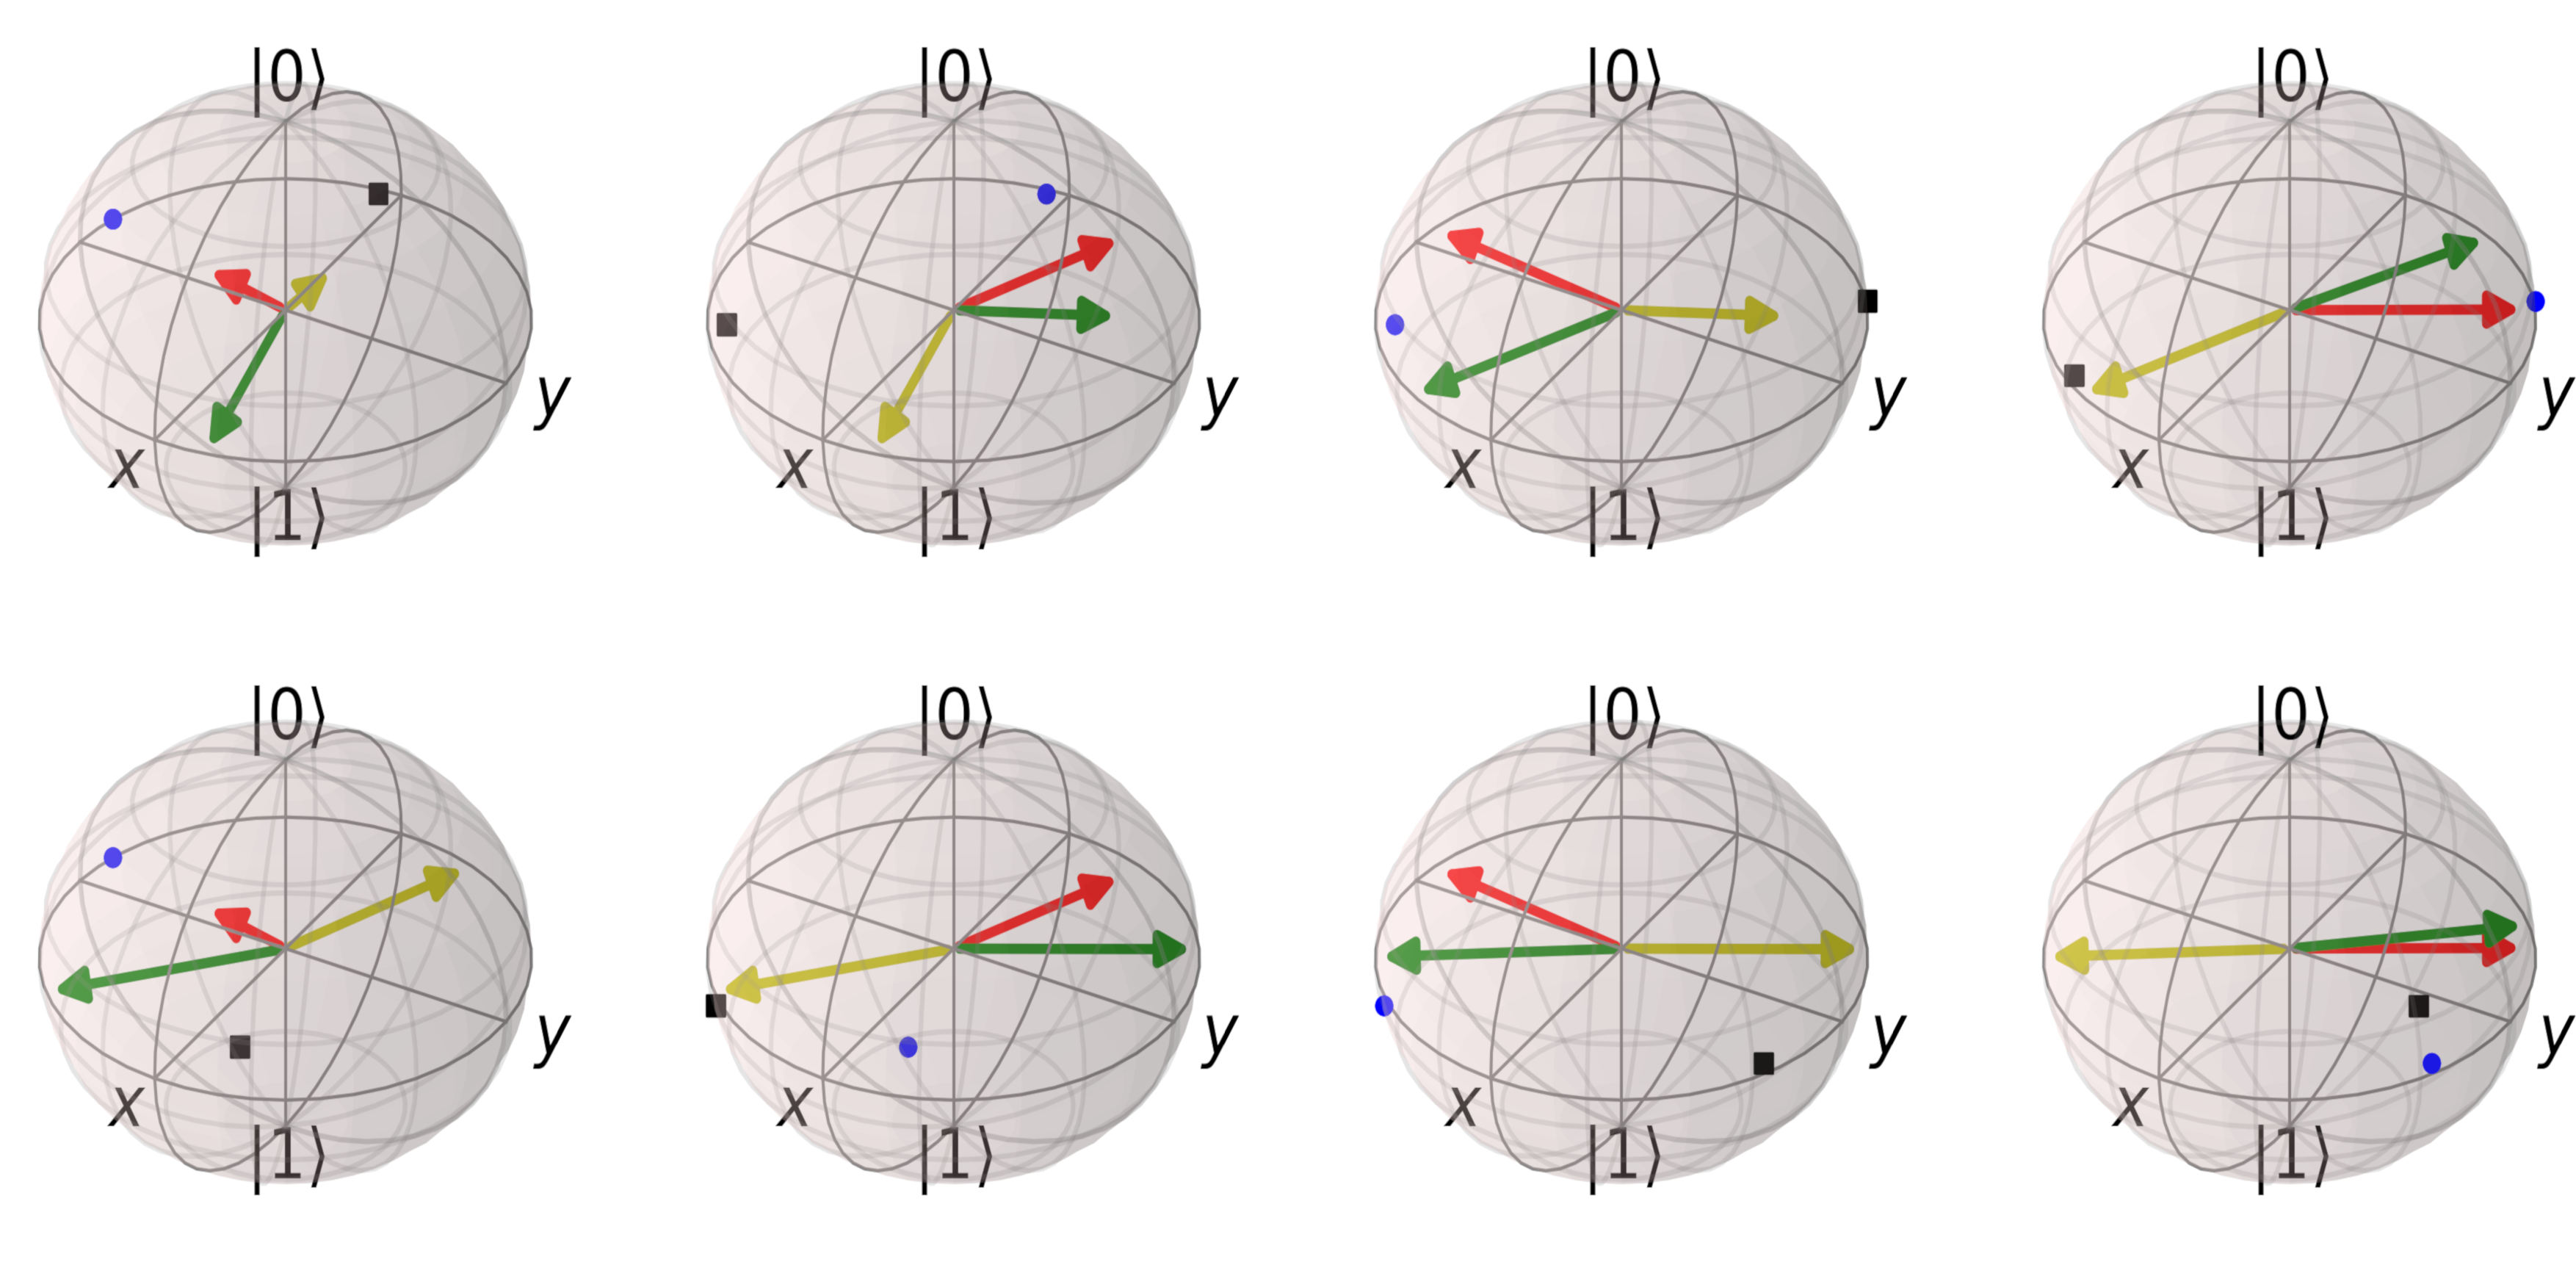
\includegraphics[width=\textwidth]{img/bloch_10553_crop_sphere2}
		\caption{$W_{opt} = 3.03, W_{pred} = 1.11$}
		\label{bloch_10553}
	\end{subfigure}
	\begin{subfigure}{0.85\textwidth}
		\centering
		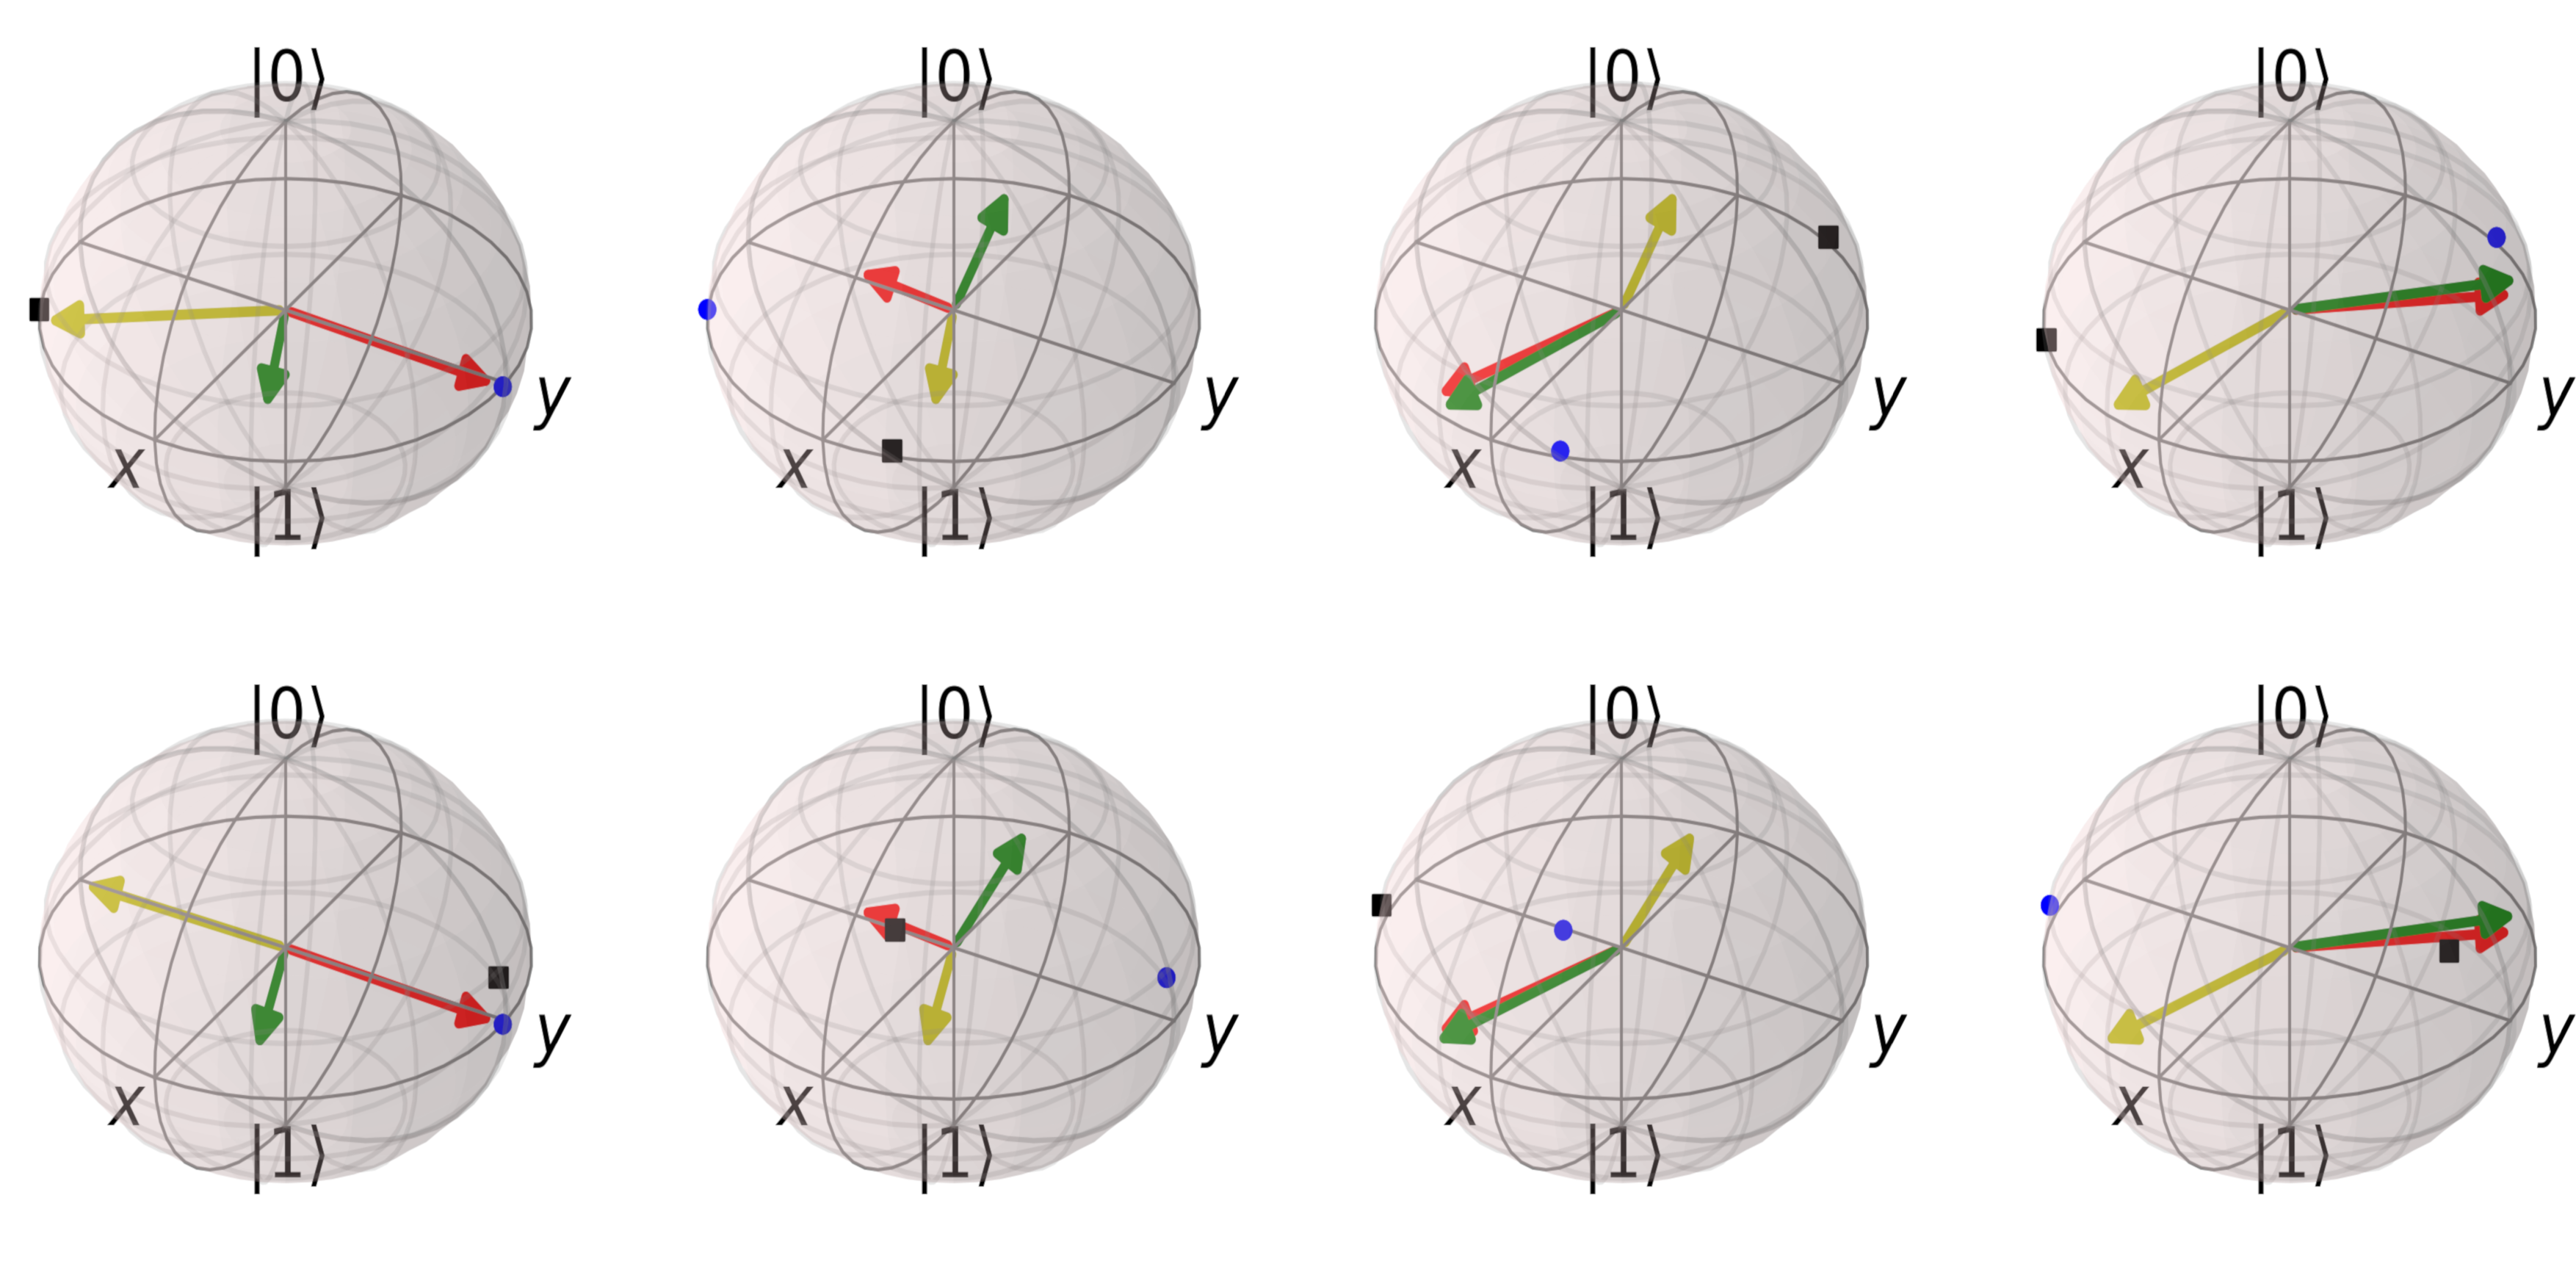
\includegraphics[width=\textwidth]{img/bloch_worst_crop_sphere2}
		\caption{$W_{opt} = 3.06, W_{pred} = -2.65$}
		\label{bloch_worst}
	\end{subfigure}
	\caption{\textbf{(a)} We plot the evolution of a sample from the test set for $N=5$ and $\Delta \mathrm{T} = 5$. Each Bloch sphere shows $\rho_S(n \Delta \mathrm{T})$ (blue dot), $\rho_S((n+1) \Delta \mathrm{T})$ (black square), the drive Hamiltonian  $H_{(D)S}^n$ (red vector) as well as $H_{S(T)}^n$ (yellow vector) and $H_{S(T)}^{n+1}$ (green vector). The Hamiltonian Bloch vectors are given by $\vec{r}_H = \Tr{H \vec{\sigma}}$. \textbf{Top row:} we plot the system dynamics for the transducer series generated by the optimiser for $n \in [1, N - 1]$. In the optimal case, $H_{S(T)}^n$ is chosen such that $\rho_S$ remains near the x-y-plane and $\Tr{\rho_S((n+1) \Delta \mathrm{T}) H_{S(T)}^n}$ is large. \textbf{Bottom row:} we plot the dynamics for the same drive protocol with transducer qubits predicted by the bidirectional LSTM. The distance of $\rho_S$ to the x-y-plane is larger. As shown in Figure \ref{bilstmbox}, $\theta_T$ is often set to $\frac{\pi}{2}$ which maximises the strength of $H^n_{S(T)}$ as can be seen in all Bloch spheres in the bottom row. In this case, $H^{n+1}_{S(T)}$ and $H^n_{S(T)}$ are chosen by the network to be antiparallel, irrespective of the current system state.
	\textbf{(b)} We show the same plot as in (a) for the worst performing sample from the test set to illustrate a shortcoming of the model. As can be seen from the yellow and green vectors, the predictions for $n \in [2, N]$ are very close to the optimal solutions (top row of (b)). However, the first transducer prediction is wrong, leading to a deviation from the optimal system dynamics.}
	\label{n_5_blochs}
\end{figure}

\begin{figure}[H]
	\centering
	\begin{subfigure}{0.45\textwidth}
		\centering
		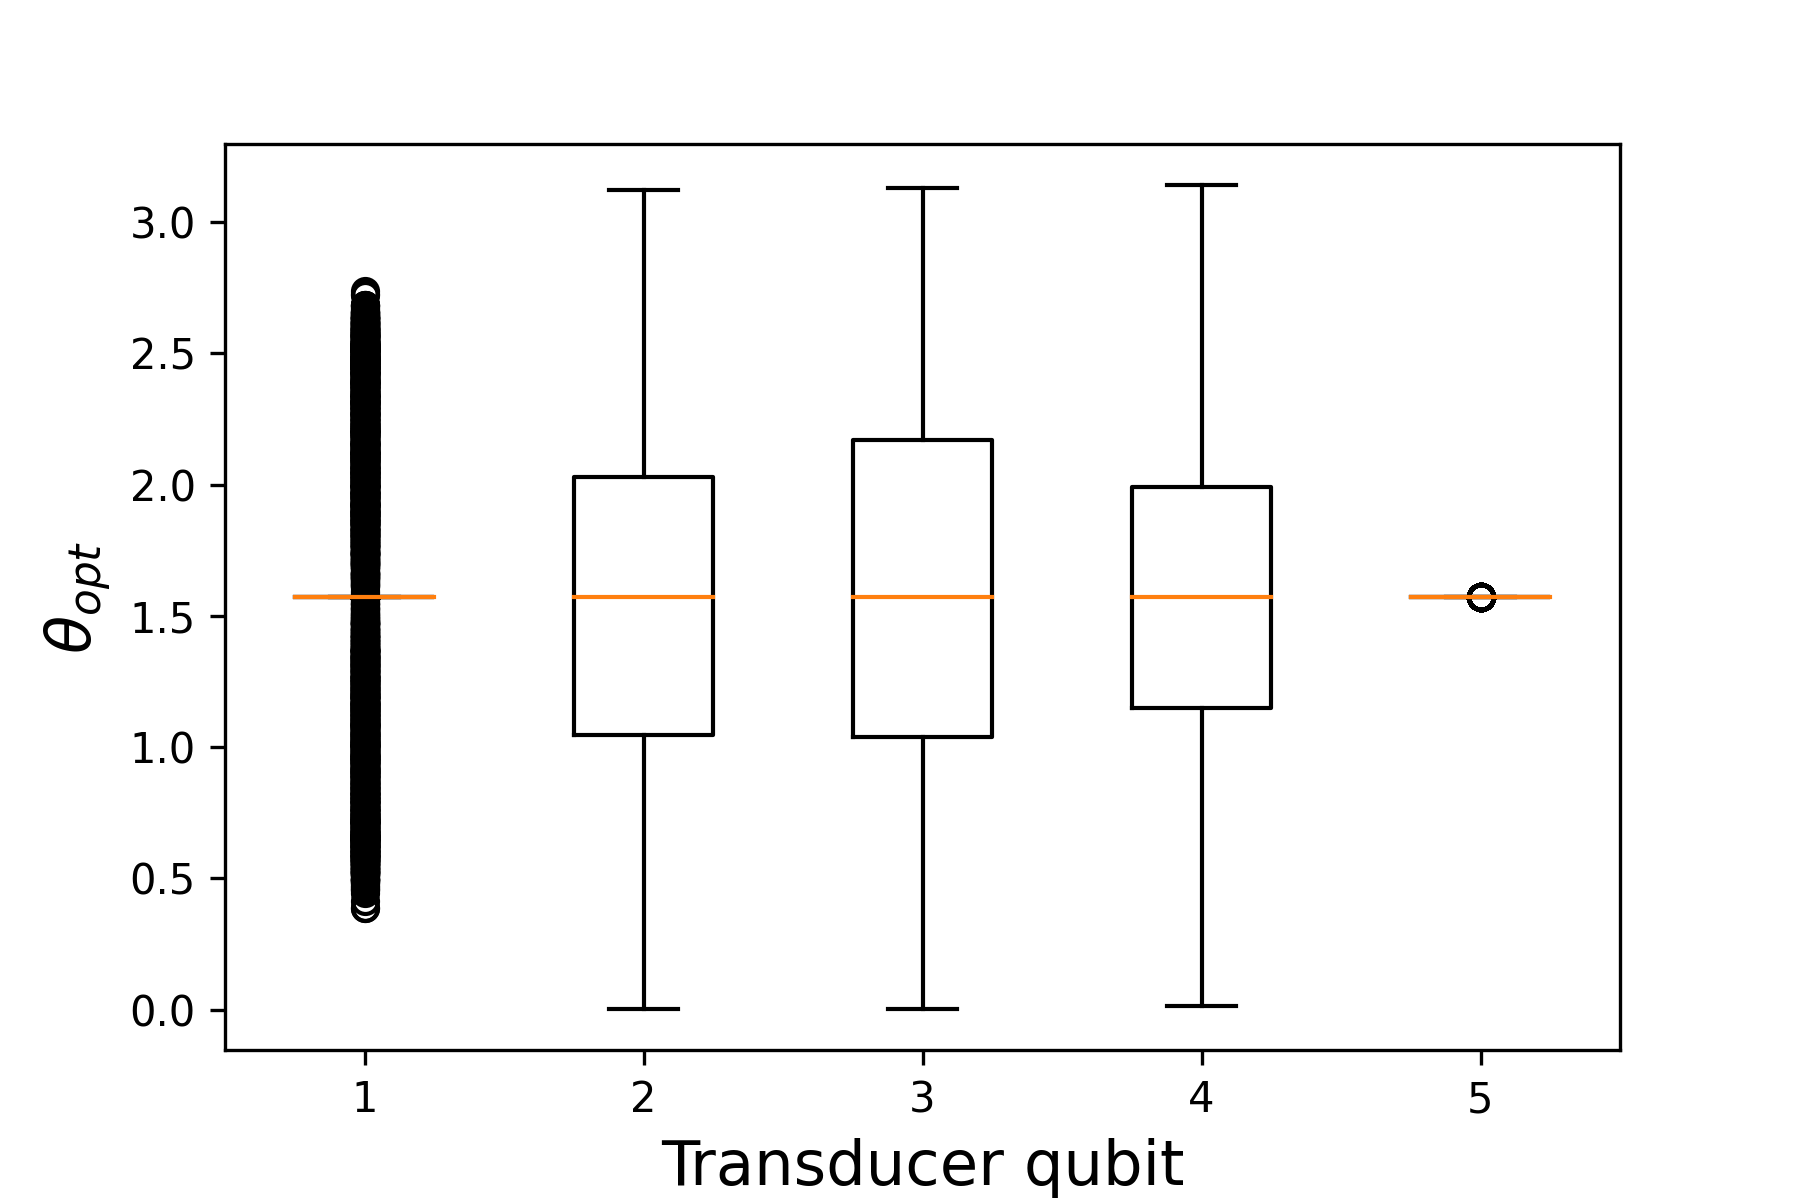
\includegraphics[width=\textwidth]{img/theta_opt_box2}
		\subcaption{$\theta^n_{\text{opt}}$}
	\end{subfigure}
	\begin{subfigure}{0.45\textwidth}
		\centering
		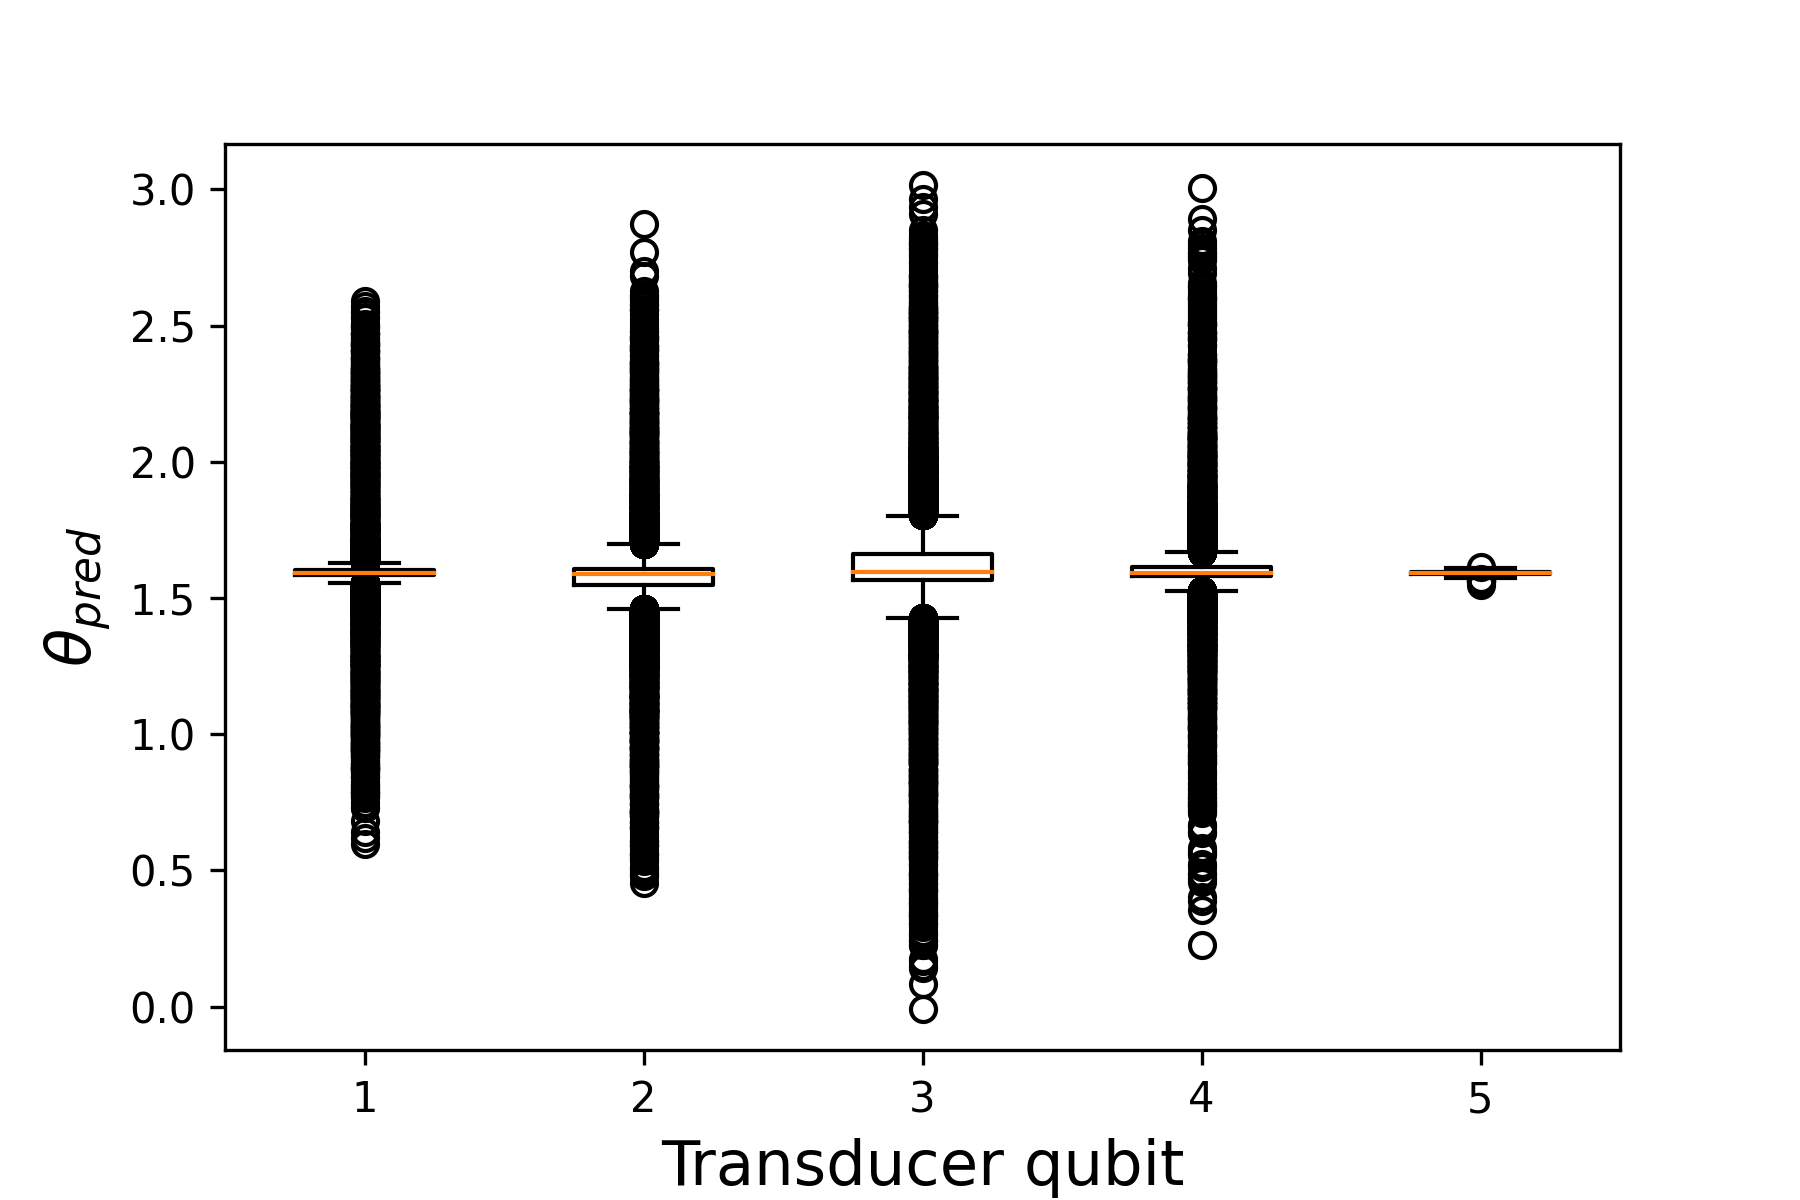
\includegraphics[width=\textwidth]{img/theta_pred_box2}
		\subcaption{$\theta^n_{\text{pred}}$}
	\end{subfigure}
	\begin{subfigure}{0.45\textwidth}
		\centering
		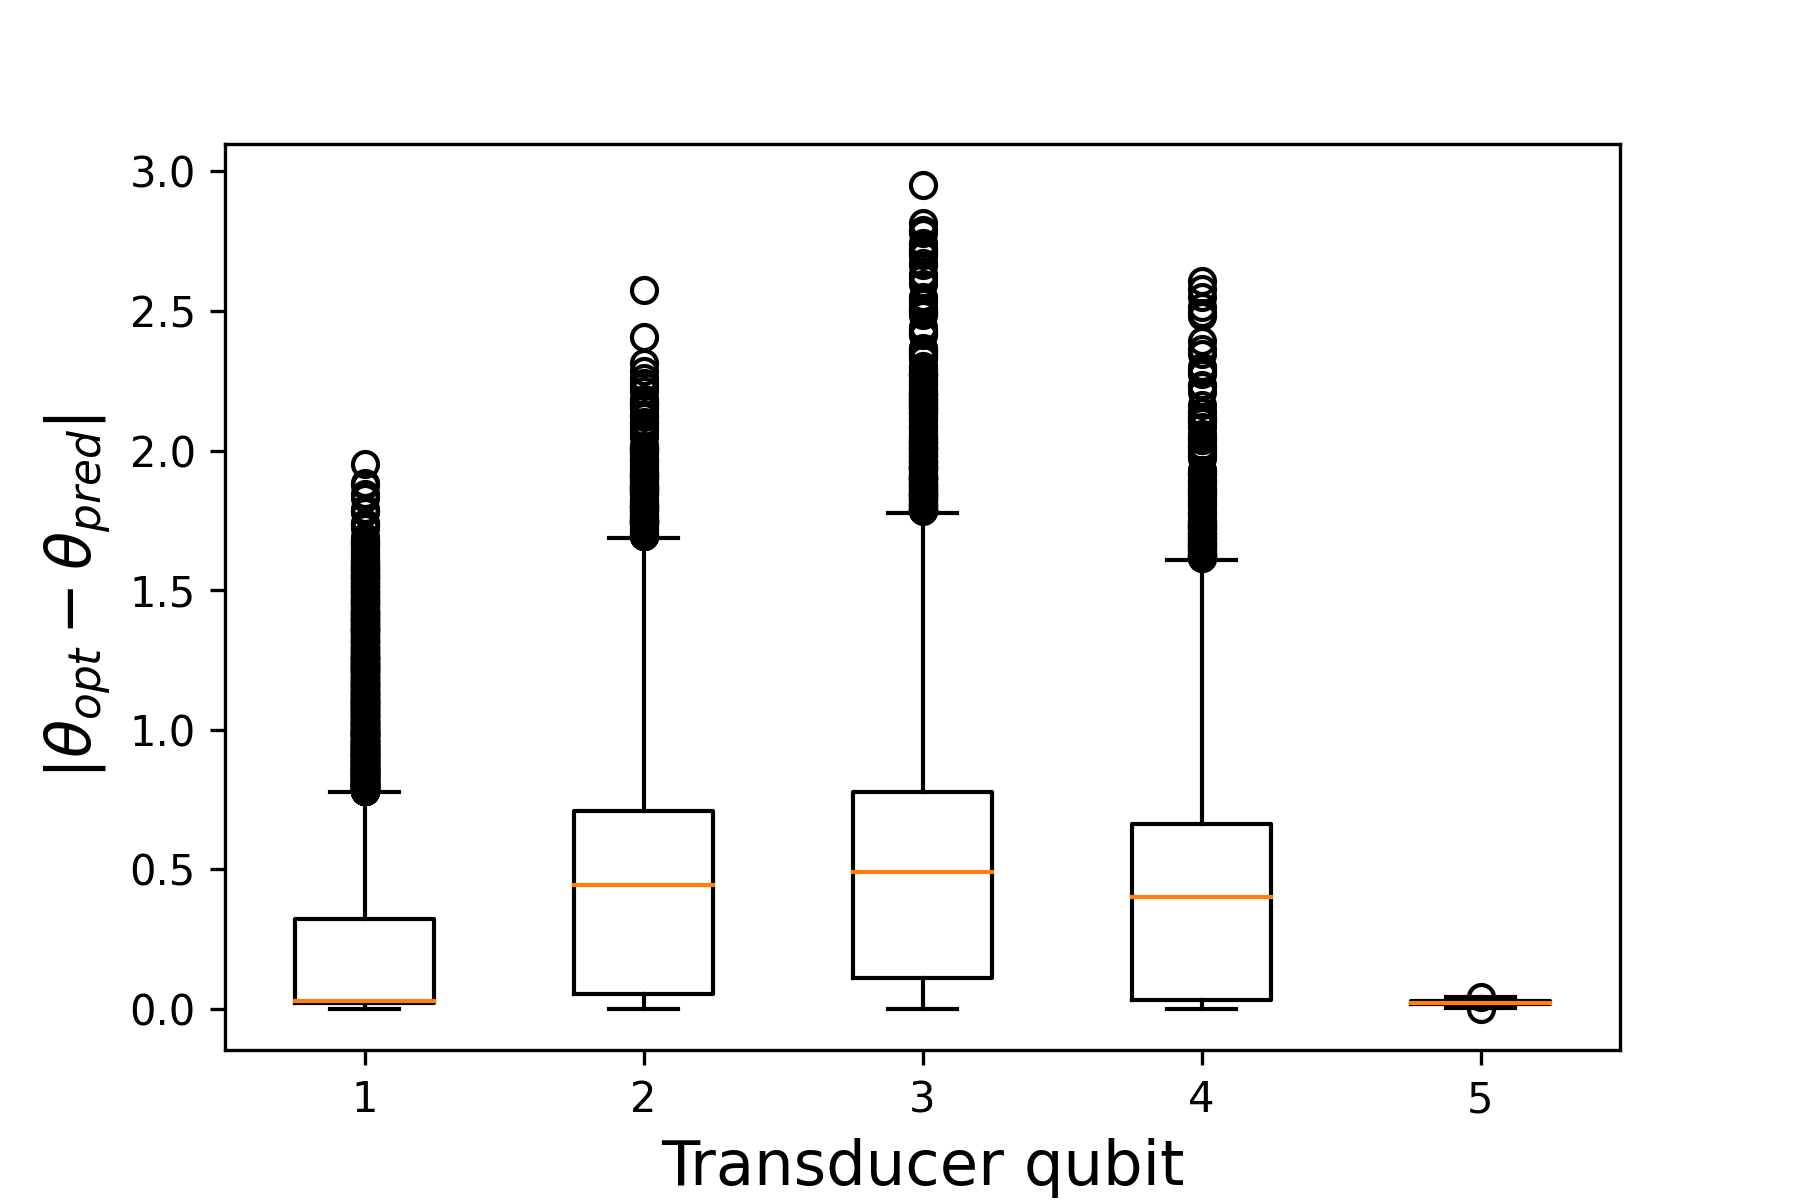
\includegraphics[width=\textwidth]{img/delta_theta_box2}
		\subcaption{$|\theta^n_{\text{opt}} - \theta^n_{\text{pred}}|$}
	\end{subfigure}
\begin{subfigure}{0.45\textwidth}
	\centering
	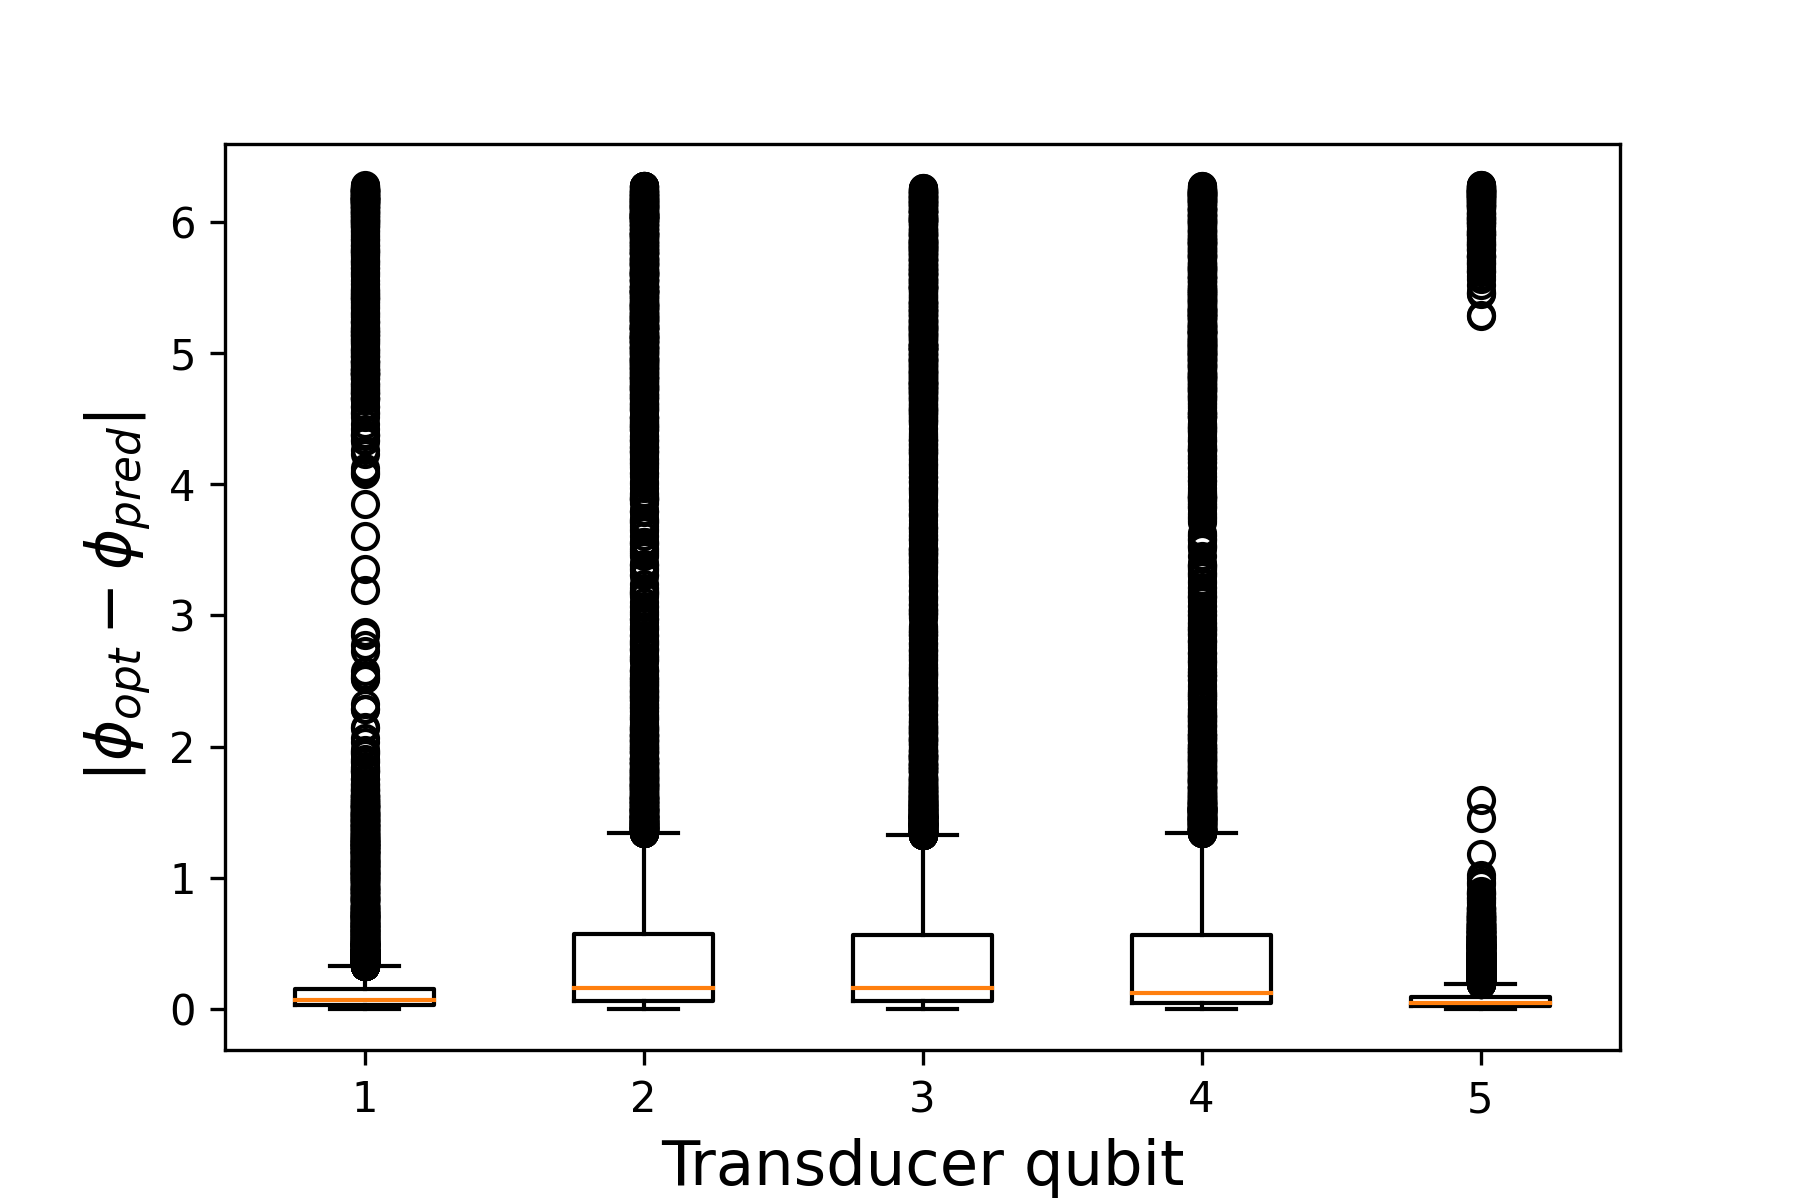
\includegraphics[width=\textwidth]{img/delta_phi_box2}
	\subcaption{$|\phi^n_{\text{opt}} - \phi^n_{\text{pred}}|$}
\end{subfigure}
\caption{For the bidirectional LSTM network and $\Delta \mathrm{T} = 5$, we plot boxplots (inside the box are values from the lower to the upper quartile (25th to 75th percentile), the orange line represents the median and the vertical lines represent the values that lie in 1.5 times the interquartile range (height of the box)) of the optimal \textbf{(a)}, predicted \textbf{(b)} and absolute differences \textbf{(c)} of $\theta^n_T$ for the five qubits of each trajectory in the test set. The prediction for $\theta_T^N$ is very good as the optimal solution is to set it to $\frac{\pi}{2}$ in all cases to maximise the work output of the final step. The prediction for $\theta_T^1$ is reasonably good too, as the optimal solution is again $\frac{\pi}{2}$ for a majority of trajectories. The network is unable to predict the three central qubits, with median absolute differences of approximately $0.5$. \textbf{(d)}: we plot the absolute difference between optimal and predicted $\phi_T^n$. We refrain from plotting the optimal and predicted $\phi_T^n$ themselves as these are distributed uniformly.}
\label{bilstmbox}
\end{figure}

\newpage